\documentclass[tikz,border=4pt]{standalone}
\usetikzlibrary{positioning, fit, backgrounds, arrows.meta}

\tikzset{
  box/.style         = {draw, thick, fill=white, text width=66mm, align=left,
                        minimum height=11mm, font=\small},
  phase/.style       = {draw=blue!40, fill=blue!5, rounded corners=2pt, inner sep=3mm},
  phase title/.style = {font=\bfseries\small, text=blue!50!black},
  >={Stealth[length=2.5mm]},
}

\begin{document}
% The PRISMA 2020 flow diagram for new systematic reviews that search
% databases and registers only. Fill in each n.
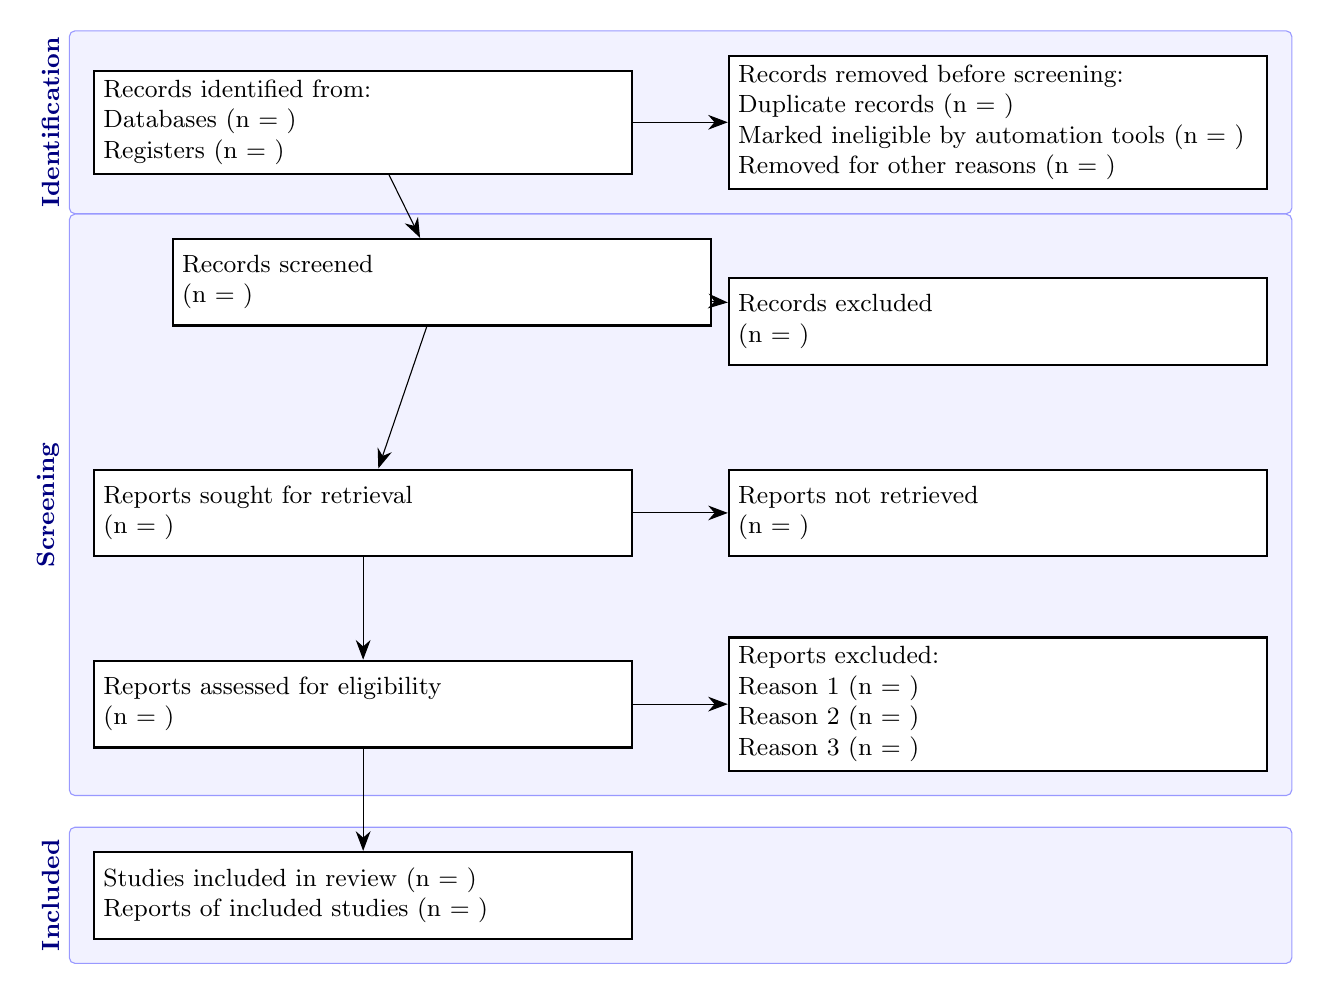
\begin{tikzpicture}[node distance=13mm and 12mm]
  \node[box] (identified) {Records identified from:\\ Databases (n = )\\ Registers (n = )};
  \node[box, right=of identified] (removed) {Records removed before screening:\\
    Duplicate records (n = )\\ Marked ineligible by automation tools (n = )\\
    Removed for other reasons (n = )};
  \node[box, below=8mm of identified, xshift=1cm] (screened) {Records screened\\ (n = )};
  \node[box, below right=1.3cm and 1.2cm of identified]   (excluded) {Records excluded\\ (n = )};
  \node[box, below=3.73cm of identified]   (sought)   {Reports sought for retrieval\\ (n = )};
  \node[box, right=of sought]     (missing)  {Reports not retrieved\\ (n = )};
  \node[box, below=of sought]     (assessed) {Reports assessed for eligibility\\ (n = )};
  \node[box, right=of assessed]   (reasons)  {Reports excluded:\\ Reason 1 (n = )\\
    Reason 2 (n = )\\ Reason 3 (n = )};
  \node[box, below=of assessed]   (included) {Studies included in review (n = )\\
    Reports of included studies (n = )};

  \draw[->] (identified) -- (removed);
  \draw[->] (identified) -- (screened);
  \draw[->] (screened)   -- (excluded);
  \draw[->] (screened)   -- (sought);
  \draw[->] (sought)     -- (missing);
  \draw[->] (sought)     -- (assessed);
  \draw[->] (assessed)   -- (reasons);
  \draw[->] (assessed)   -- (included);

  \begin{scope}[on background layer]
    \coordinate (lanes left) at (identified.west);
    \coordinate (lanes right) at (removed.east);
    \node[phase, fit=(identified) (removed) (identified -| lanes left) (identified -| lanes right),
          label={[phase title, rotate=90, anchor=south]west:Identification}] (identification) {};
    \node[phase, fit=(screened) (excluded) (sought) (missing) (assessed) (reasons)
            (screened -| lanes left) (screened -| lanes right),
          label={[phase title, rotate=90, anchor=south]west:Screening}] (screening) {};
    \node[phase, fit=(included) (included -| lanes left) (included -| lanes right),
          label={[phase title, rotate=90, anchor=south]west:Included}] (inclusion) {};
  \end{scope}
\end{tikzpicture}
\end{document}
